% ---------------------------------------------------
% ----- Chapters of the template
% ----- for Bachelor-, Master thesis and class papers
% ---------------------------------------------------
%  Created by C. Müller-Birn on 2012-08-17, CC-BY-SA 3.0.
%  Freie Universität Berlin, Institute of Computer Science, Human Centered Computing. 
%
\chapter{Kapitel}
\label{chap:chapters} 

%\begin{itemize}
	%\item Abhängig vom Ziel der Arbeit und dem verwendeten Forschungsdesign
	% unterscheidet sich dieser Hauptteil der Arbeit erheblich.
	%\item Eine sehr allgemeine Struktur ist die folgende:
	%\begin{itemize}
		%\item Hintergrund der Arbeit (Theoretische Einordnung der Arbeit)
		\section{Hintergrund der Arbeit}
		\subsection{Mapping Methoden}
		Der grundlegende Prozess für die Bestimmung möglicher Matches von Eigenschaften
		sieht wie in Abbildung \ref{fig1} gezeigt aus. Das zentrale Element dabei ist
		der Matcher. \cite{Hoo14}
		
		\begin{figure}[ht]
		\centering
		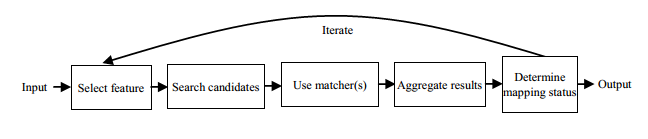
\includegraphics[width=1.0\textwidth]{simple-high-level-view-of-a-mapping-process.png}
		\caption{Eine einfache Übersicht des Mapping Prozesses \cite{Hoo14}}
		\label{fig1}
		\end{figure}
		
		Im ersten Schritt wird ein Element (\textit{feature}), wie ein Label für
		Entitäten oder Instanzen von Attributen, aus einer der zu matchenden Ontologien ausgewählt,
		anschließend werden in der anderen Ontologie nach möglichen, passenden
		Elementen (sogenannte \textit{candidates}) gesucht. Mithilfe der Matcher werden
		die beiden Eigenschaften dann verbunden, sofern der oder die Matcher Übereinstimmungen vermuten. Die Ergebnisse werden dann zusammengefasst und zum Schluss entweder in einer neuen Iteration berücksichtigt oder ausgegeben. \cite{Hoo14}\\
		Neben der direkten Verbindung kann man die Eigenschaften aus den Ontologien, die
		gematched werden sollen, über sogenannte \textit{Anker} (Anchors) mit einer
		weiteren Ontologie verbunden, deren Zweck es ist, als „Meta-Ontologie“ eine gemeinsame Schnittstelle zu bilden. Anker sind Entitäten, die als gleichartig zu Entitäten der anderen Ontologien definiert werden. \cite{Hoo14}
		
		\subsection{Kategorien von Matchern}
		Um Ontologien zu matchen gibt es verschiedene Möglichkeiten. Diese können einzeln, aber auch kombiniert auf verschiedene Weise angewendet werden. Eine Möglichkeit ist es, mehrere Matcher sequentiell anzuwenden, um die Ergebnisse immer mehr zu verfeinern und zu verbessern. Eine andere Variante ist es, mehr als eine Matching Methode parallel anzuwenden und dann die Ergebnisse zusammenzufügen. Diese beiden Aggregationsverfahren kann man auch kombinieren. \cite{Hoo14}
		
		\subsection{Terminologisches Mapping}
		Um Elemente von Ontologien zu matchen, kann man deren Benennung durch Tokenisierung in ein gemeinsames Format überführen und dann mithilfe von Gewichtung und Gleichheit in Relation setzen.
		\begin{itemize}
			\item Stringbasiert: Bei dieser Methode wird die Struktur von Strings als
			Zeichenketten betrachtet. Konkret werden Techniken angewendet, die Ähnlichkeit von Strings und deren Teilen bestimmen. Bekannte Methoden aus diesem Bereich sind z.B. Normalisierung und Editierdistanz. \cite{Euz07}  Beispielsweise beträgt der Abstand der Elemente „author“ und „hasauthor“ 3, nämlich den Zusatz „has“, sofern der Algorithmus erkennt, dass der hintere Teil gleich ist.
			\item  Sprache basiert: Hierbei werden Wörter als Texte betrachtet, d.h. die
			Reihenfolge der Wörter in einer Sequenz wird einbezogen, ebenso die Bedeutung dieser Wörter. Zur Analyse werden verschiedene Techniken angewandt, um das Grundwort zu ermitteln. Dieses dient dann dazu, Ähnlichkeiten zwischen den Wörtern zu finden. \cite{Euz07}  Zum Beispiel, wenn man in einer Ontologie das Element „walk“ und in einer anderen „walking“ hat, kann man „walking“ auf „walk“ reduzieren (z.B. durch Stemming) und dadurch Matches finden.
			\item Linguistische Analyse: Durch das Einbeziehen von externen
			linguistischen Quellen, wie z.B. Wiktionary , werden Strings interpretiert.
			Beim bedeutungsbasierten Ansatz werden über \textit{Hyponyme} (begriffliche
			Unterordnung), \textit{Hyperonyme} (Ober-/Überbegriff), \textit{Synonyme}
			(gleiche Bedeutung) und \textit{Antonyme} (gegensätzliche Bedeutung) die
			Bedeutung der Wörter festgestellt. Beim sprachbasierten Ansatz hingegen, wird der Abstand zu anderen Wörtern in Sätzen analysiert. \cite{Euz07} Zum Beispiel kann man „creator“ als Oberbegriff von „author“ und „illustrator“ auffassen.
		\end{itemize}
		
		\subsection{Strukturelles Mapping}
		Eine zweite Möglichkeit für das Matching von Ontologien ist das Betrachten der Strukturen innerhalb der Ontologien. Dabei werden die Eigenschaften und die Beziehung der Entitäten untereinander untersucht.
		\begin{itemize}
			\item Taxonomisches Mapping: Dabei werden zwei Techniken verwendet, super-
			oder  subclass rule und bounded-paths. Die super class rule unterstellt, dass eine Ähnlichkeit zwischen zwei Konzepten besteht, wenn diese ein Elternkonzept teilen. \cite{Euz07}  Beispielsweise kann man annehmen, dass wenn zwei Ontologien ein gleiches oder ähnliches Konzept haben, um Bücher zu beschreiben, dass die darunterliegenden Konzepte für die Beschreibung für „creator“ und „author“ ebenfalls ähnlich bzw. gleich sind. Bei bounded-paths werden Pfade verglichen, um ähnliche Konzepte zu identifizieren. Bei diesen Pfaden handelt es sich um Verbindungen zwischen Klassen. Die Art und Weise der Verbindungen wird durch eine hierarchische Struktur definiert. \cite{Euz07} Wenn das Attribut „book“ in zwei verschiedenen Ontologien einmal mit „hasAuthor“ und einmal mit „hasWritten“ zu den beiden äquivalenten Elementen „creator“ bzw. „author“ verbunden ist, dann bieten sich diese beiden für eine Betrachtung bezüglich eines Matches an.
			\item Baumbasiertes Mapping: Hierbei spielt Ähnlichkeit eine Rolle. Es wird
			angenommen, dass sich Knoten ähneln, die benachbart sind, und dass dies auch für verschiedene Ontologien gilt. Also wenn ein Knoten mit einem anderen benachbart ist und mit einem Knoten aus einer anderen Ontologie verbunden ist, dann ähneln sich die benachbarten Knoten mit den beiden verbundenen. Wenn beispielsweise in einer Ontologie das Element „book“ über „author“ mit „human“ verbunden ist und in einer zweiten Ontologie „volume“ über „author“ mit „writer“, wobei festgelegt wurde, dass sowohl „book“ und „volume“, als auch die beiden „author“ Elemente äquivalent sind, besteht Grund zur Annahme, dass „human“ und „writer“ ebenfalls ähnlich sind. \cite{Euz07} 
		\end{itemize}
		
		\subsection{Recommender Systems}
		Als Recommender Systeme werden Software und Techniken bezeichnet, die dazu
		dienen, ihren Anwendern sinnvolle Vorschläge bezüglich Entscheidungen zu machen. Meist sind diese Systeme darauf hin ausgerichtet, unerfahrene oder nicht sachkundige Nutzer zu unterstützen. \cite{Fra10}  Bekannt sind den meisten Menschen solche System überwiegend aus den Bereichen des eCommerce, wo sie genutzt werden, um Kunden oder Besuchern Produkte vorzuschlagen, die diese interessieren könnten.\\
		In ihrer einfachsten Form, werden möglich Vorschläge in einer Liste gesammelt und dann entsprechend der Präferenzen des Nutzers und (Rand-)Bedingungen geordnet. Beide ergeben sich direkt, z.B. beim Ansehen eines Produkts in einem Webshop, oder indirekt, z.B. über die Empfehlung eines Films des gleichen Regisseurs. \cite{Fra10} 
		
		\subsection{Information Visualization}
		Bei der Information Visualization geht es im Kern darum, Daten grafisch
		darzustellen. Dadurch ist es möglich, Daten anzuzeigen, um den
		Nutzer bzw. Betrachter nicht das Interesse verlieren zu lassen. Weiterhin ermöglichen eine gute Aufbereitung der Daten und ein
		gutes User Iterface (UI) ein leichteres Navigieren innerhalb dieser Daten und deren Verknüpfung.\\
		Dafür gibt es eine Reihe an Techniken, um dies zu bewerkstelligen. Die
		Visualisierung von Informationen ist eng verknüpft mit der \textit{visuellen
		Datenexploration} (visual data exploration).
		Bei der visuellen Datenexploration werden Daten visualisiert, um es Menschen zu
		ermöglichen, diese Daten zu durchdringen, Schlüsse aus ihnen zu ziehen und direkt mit den Daten zu interagieren. \cite{Kei02}\\ Die manuelle Exploration von Daten kann zum Generieren von Hypothesen auf Basis von Daten genutzt werden, zusätzlich zur Anwendung von automatisierten Techniken aus der Statistik oder Machine Learning. Da diese beiden Arten von Techniken nicht immer anwendbar sind, kann man trotzdem gute Ergebnisse bei der Auswertung erzielen. Insbesondere wenn es  sich um stark inhomogene oder stark verrauschte Daten handelt. Zusätzlich kann man Datenexploration oft auch dann durchführen, ohne tiefgreifendes Verständnis von komplexen  mathematischen oder statistischen Algorithmen oder Parametern zu haben. \cite{Kei02} 
		
		\section{Vorhandene Software}
		Da es bereits Software für den Umgang mit Ontologien und das Matchen derselben gibt, wird sie an dieser Stelle betrachtet. Zum einen, um das Rad in diesem Bereich nicht neu und möglicherweise schlechter zu erfinden, sondern zu erweitern und/oder andere Aspekte zu behandeln. Und zum anderen soll von bestehenden Tools gelernt werden. Da die Auswahl an möglichen Tools groß ist \cite{Ber14} , können nicht alle in diesem Rahmen ausführlich vorgestellt werden. Daher erfolgt hier nur eine Auswahl. Reine Frameworks wurden bei der Bewertung nicht beachtet, da diese für die Zielgruppe nicht technischer Experten nicht geeignet sind, sondern für Entwickler von entsprechenden Tools.
		
		\subsection{AgreementMakerLight}
		\textit{AgreementMakerLight} ist ein automatisiertes Ontologie Matching System,
		das eine Weiterentwicklung der Software AgreementMaker ist und seit Anfang 2013 entwickelt wird. Der AgreementMakerLight ist Open Source , wird unter der Apache Lizenz Version 2.0 veröffentlicht und kann daher frei weiterentwickelt und verwendet werden. Es ist ein erweiterbares Framework und will Probleme bei umfangreichen Ontologie Matchings durch Effizienz angehen. Hauptsächlich finden Techniken Anwendung, die auf Elementebene arbeiten und durch domänspezifisches Wissen ergänzt werden.
		Der AgreementMakerLight wird als vorbereitetes Projekt für die Integrated
		Development Environment (IDE) Eclipse und als ausführbares Java-Archiv (jar) angeboten. Beides trifft die gewählte Zielgruppe aber nicht. Als Projekt ist es eher für Entwickler oder zumindest mit Softwareentwicklung vertrauten Personen gerichtet. Um eine jar-Datei auszuführen, ist eine Installation von Java nötig, was dem Gedanken des im Rahmen dieser Arbeit zu erstellenden Tools widerspricht, unkompliziert und sofort benutzbar zu sein.
		
		\subsection{PARIS}
		\textit{PARIS}, kurz für Probabilistic Alignment of Relations, Instances, and
		Schema, ist ein System, um Ontologien im RDF Format zu matchen. Dabei werden Verbindungen
		auf Instanz- und Klassenebene gesucht und wirken sich aufeinander aus. Matchings wird eine Wahrscheinlichkeit zugerechnet, um ohne das Festlegen von Parametern zu arbeiten. In Tests mit großen Ontologien erzielt PARIS eine Trefferquote von etwa 90\%. PARIS steht unter einer Creative Commons Lizenz , die eine kommerzielle Nutzung untersagt und eine Namensnennung der Ersteller vorschreibt. Ansonsten ist die Erweiterung und Nutzung aber frei\\
		PARIS wird neben dem reinen Quellcode als jar-Datei ausgeliefert. Wie beim AgreementMakerLight ist dies für die Zielgruppe kein idealer Anwendungsfall. Weiterhin wird PARIS über die Kommandozeile gestartet, im Gegensatz zu z.B. AgreementMakerLight, was eine zusätzliche Hürde darstellt.
		
		\subsection{COMA 3.0}
		\textit{COMA 3.0} ist Matching Tool für Schemata und Ontologien und wurde am
		Institut für Informatik an der Universität Leipzig entwickelt. Es gibt sowohl eine klassische Software- als auch eine Webversion. Beide wurden in Java entwickelt. Die Webversion wird als Java Applet angeboten. Die Vorgänger von COMA 3.0 hießen COMA und COMA++ und es ist eine Weiterentwickelung von diesen. Dafür wurden das Management des Workflows verbessert und Features hinzugefügt, darunter Ontologie Matching.
		Da die im Rahmen dieser Mastarbeit entwickelte Software als Webapplikation entwickelt werden soll, wird wegen der Ähnlichkeit nur das Java Applet betrachtet. Als Java Applets wird Java Software in Java Bytecode bezeichnet, die über einen Webbrowser ausgeführt werden kann.  Dafür werden in Browsern Plug-Ins benötigt, die in der Regel aber nicht vorinstalliert sind. Auch gab es immer wieder Probleme mit Sicherheitslücken und „das Java-Plug-in war als einer der größten Türöffner für Sicherheitsangriffe bekannt und wurde in Untersuchungen immer wieder als Risiko Nummer eins auf den PCs dieser Welt bezeichnet“.  Zu Beginn des Jahres 2016 wurde von Oracle, dem Hersteller von Java, verkündet, dass diese Technologie nicht mehr weiterentwickelt wird.  Weiterhin ist die Portabilität über Betriebssysteme nicht unproblematisch, da Browser auf mobilen Geräten, die Plug-Ins fast ausnahmslos nicht unterstützen.  Das sind alles Gründe, die gegen einen Einsatz im Benutzerkreis sprechen, der im Rahmen dieser Mastarbeit angesprochen werden soll.
		
		\subsection{LODE}
		\textit{LODE} (Linked Open Data Enhancer) ist ein webbasiertes Tool, um
		Ontologien zu erkunden, zu matchen und zu erweitern. Es ist Open Source  und wird innerhalb des Play Frameworks   verwendet. Entwickelt wurde es in der Kooperation der Universitäten Mannheim, Washington und Indiana.
		
		\subsection{HerTUDA}
		\textit{HerTUDA} ist ein Ontologie Matching Tool der Knowledge Engineering
		Arbeitsgruppe des Fachbereichs Informatik an der Technischen Universität Darmstadt. Es ist auf schnelles und einfaches Arbeiten ausgelegt und arbeitet mit syntaktischen Vergleichen von Strings und Herausfiltern irrelevanter Matches.
		 		%\item Hier sollte enthalten sein, welche Anwendungen in diesem Bereich
		 		% bereits existieren und warum bei diesen ein Defizit besteht.
				%\item Falls genutzt, sollten hier die entsprechenden Algorithmen erläutert
				% werden.
				%\item Es sollten die Ziele der Anwendungsentwicklung, d.h. die
				% Anforderungen herausgearbeitet werden. Dabei sollte die bestehende Literatur geeignet integriert werden.
		 	%\end{itemize}
		%\item Umsetzung (Praktischer Anteil der Arbeit)
		%\item Umsetzung (Praktischer Anteil der Arbeit)
			%\begin{itemize}
				%\item Zunächst sollte die Softwarearchitektur und die genutzten
				% Anwendungen, APIs etc. erläutert werden. Ebenfalls gehört dazu das Datenbankschema.
				%\item Es sollten die zentralen Elemente der Software (abhängig von der
				% Aufgabenstellung) beschrieben werden, wie implementierte Algorithmen oder das Oberflächendesign.
				%\item Zentraler Quellcode sollte entsprechend aufgelistet werden:
				%\lstset{language=Java,basicstyle=\footnotesize,numbers=left,showstringspaces=false,frame=single}
				%\begin{lstlisting}
				%public class Main {
				%	public static void main(String[] args) {
				%		System.out.println("Hello World!");
				%	}
				%}
				%\end{lstlisting} 
				%\item Klassendiagramm für Backend
				%\item Dr Quellcode zentraler Implementierungen  können als Auszug in den Anhang. Im Text kann dann darauf verwiesen werden.
			%\end{itemize}
		%\item Evaluation (zumeist nur für Masterarbeiten relevant)
		%\begin{itemize}
		%	\item Jede Software muss auch getestet werden. Dieses Tests werden entweder
			% mit einem vorgegebenen Datensatz erfolgen oder aber die Evaluation erfolgt auf Basis von Experimenten. In diesem Kapitel sollte daher entweder der genutzte Datensatz oder der experimentelle Aufbau beschrieben werden.
		%\end{itemize}
		%\item Ergebnis und Diskussion
		%\begin{itemize}
		%	\item Die Ergebnisse der Anwendung werden in diesem Kapitel vorgestellt und
			% anschließend diskutiert. Wenn möglich sollte die Ergebnisse in Relation zu bestehenden Arbeiten in dem Bereich erörtert werden.
		%\end{itemize}
	%\end{itemize}  
%\end{itemize}